\chapter{Control 1: Derivada numérica y error máximo}\label{ch:Control1}


\hfill \textbf{Fecha de la actividad:} 17 de septiembre de 2024

\medskip

En este capítulo, revisaremos los ejercicios planteados en el control 1 del miércoles 4 de septiembre de 2024.

Usaremos métodos de trabajo con funciones diferenciales y estimación de error

\begin{definition} \textbf{Función diferencia}\\
Sea $f:D\subseteq\mathbb{R}^n\to\mathbb{R}^m$

Se define el diferencial de $f$ en $h$, como:
\begin{align*}
    \delta_{f}&:D\times D_x\to\mathbb{R}^m\\
    \delta_{f}&(x,h)=f(x+h)-f(x)
\end{align*}
donde $D_x=\{h\in\mathbb{R}^n:h+x\in D\}$ es el dominio $D$ tal que $\delta_{f(x)}(0)=0$, es decir, con $0$ en $x$
\end{definition}
\begin{theorem}
    Sea $f:D\subseteq\mathbb{R}\to\mathbb{R}$ analítica.
    
    Entonces:
    \begin{align*}
        \delta_{f(x)}(h)=\sum_{n=1}^\infty f^{(n)}(x)\frac{h^n}{n!}
    \end{align*}
\end{theorem}
En teoría de la computación, no podemos computar infinitos términos, así que solo computamos hasta el término $n$, y luego consideramos una función de error en $h$ una función del error de truncamiento.
\begin{align*}
    \delta_{f}(x,h)=\sum_{i=1}^n f^{(i)}(x)\frac{h^{i}}{i!} + h^{n+1}\mathcal{E}(h)
\end{align*}
donde pedimos que
\begin{align*}
    \lim_{h\to 0} \mathcal{E}(h)=\lim_{h\to 0}\frac{\delta_f(x,h)-\sum_{i=1}^n f^{(i)}(x)\frac{h^{i}}{i!}}{h^{n+1}}=0
\end{align*}
Si hacemos combinaciones lineales en $h$ de $\delta_f$, entonces podemos reducir el error, al coste de más terminos a evaluar
\newpage
\begin{exercise}
\begin{align*}
    f''_{num}(x,h)=\frac{-3f(x)+f(x-2h)+2f(x+h)}{3h^2}
\end{align*}
Encuentra su error
\end{exercise}

Para abordar este problema, encontremos las funciones en términos de las funciones diferenciales.
\begin{align*}
    2\delta_f(x,h)&=2(f(x+h)-f(x))\\
    &=2\left(f'(x)h+\frac{f''(x)h^2}{2}+h^3\mathcal{E}_1(h)\right)\\
    \delta_f(x,-2h)&=f(x-2h)-f(x)\\
    &=f'(x)(-2h)+\frac{f''(x)(2h)^2}{2}+h^3\mathcal{E}_2(h)\\
    \implies 2\delta_f(x,h)+\delta_f(x,-2h)&=-3f(x)+2f(x+h)+f(x-2h)\\
    &=6f''(x)\frac{h^2}{2}+h^3\mathcal{E}(h)
\end{align*}
Luego:
\begin{align*}
    f''(x)=\frac{2\delta_f(x,h)+\delta_f(x,-2h)}{3h^2}-\frac{h}{3}\mathcal{E}(h)
\end{align*}

Finalmente, el error de $f''_{num}(x,h)=h\mathcal{E}(h)$, donde:
\begin{align*}
    \mathcal{E}&=\mathcal{E}_1+\mathcal{E}_2\\
    &=\left(\frac{2}{3!}f^{(3)}(x)+\frac{2}{4!}f^{(4)}(x)h+\dots\right)\\
    &+\left(\frac{(-2)^3}{3!}f^{(3)}(h)+\frac{(-2)^4}{4!}f^{(4)}(x)h+\dots\right)\\
    &=f^{(3)}(x)+\frac{18}{24}f^{4}(x)h+\dots
\end{align*}
Por el Teorema del Valor Medio (TVM), existe un único $\xi \in [x,x+h]:f^{(3)}(\xi)=\mathcal{E}(h)$. Luego:
\begin{align*}
    f''(x)=f''_{num}(x,h)-\frac{h}{3}f'''(\xi)
\end{align*}
\begin{exercise}
    Si realizamos computaciones numéricas en un programa, las cuales poseen un error de redondeo, obtenga el error total $E$
    \begin{align*}
        E(h)=\left|f''(x)-f''_{num}(x,h)\right|
    \end{align*}
    De modo que el gráfico de $(h,E(h))$ esté acotado superiormente.
\end{exercise}
Aquí, tenemos que definir el error de redondeo. Sea
\begin{align*}
    \bar{A}=A(1+\varepsilon)
\end{align*}
la aproximación de $A$ calculado por el computador. Así:
\begin{align*}
    \bar{E}(h)&=\left|\bar{f}''(x)-\bar{f}''_{num}(x,h)\right|\\
    &=\left|\frac{-h}{3}f'''(\xi)+f''(x)\varepsilon_1+f''_{num}(x)\varepsilon_2\right|\\
    &\leq \frac{h}{3}|f'''(\xi)|+|f''(x)\varepsilon_1|+|f''_{num}(x,h)\varepsilon_2|
\end{align*}
Ahora, debemos recordar las definiciones originales de $f''$ y $f''_{num}$
\begin{align*}
    |f''(x)\varepsilon_1|&=\left|\frac{-3f(x)}{3h^2}+\frac{2f(x+h)}{3h^2}+\frac{f(x-2h)}{3h^2}-\frac{h}{3}f'''(\xi)\right||\varepsilon_1|\\
    &\leq \left|\frac{f(x)\varepsilon_1}{h^2}\right|+\frac{2}{3}\left|\frac{f(x+h)\varepsilon_1}{h^2}\right|+\frac{1}{3}\left|\frac{f(x-2h)\varepsilon_1}{h^2}\right|+\frac{h}{3}\left|f'''(\xi)\varepsilon_1\right|\\
    |f''_{num}(x)\varepsilon_2|&=\left|\frac{-3f(x)}{3h^2}+\frac{2f(x+h)}{3h^2}+\frac{f(x-2h)}{3h^2}\right||\varepsilon_2|\\
    &\leq \left|\frac{f(x)\varepsilon_2}{h^2}\right|+\frac{2}{3}\left|\frac{f(x+h)\varepsilon_2}{h^2}\right|+\frac{1}{3}\left|\frac{f(x-2h)\varepsilon_2}{h^2}\right|
\end{align*}
Si $h\to dh \implies \xi \to x$, esto es, si aproximamos con un $h$ lo suficiente pequeño, el error de evaluar $\xi$ como $x$ es despreciable.\\
Por otra parte: $\forall \lambda: x+\lambda h\to x$. Luego:
\begin{align*}
    \bar{E}(h)&\leq \frac{h}{3}|f'''(x)|\\
    &+\left|\frac{f(x)\varepsilon_1}{h^2}\right|+\frac{2}{3}\left|\frac{f(x)\varepsilon_1}{h^2}\right|+\frac{1}{3}\left|\frac{f(x)\varepsilon_1}{h^2}\right|+\frac{h}{3}\left|f'''(x)\varepsilon_1\right|\\
    &+\left|\frac{f(x)\varepsilon_2}{h^2}\right|+\frac{2}{3}\left|\frac{f(x)\varepsilon_2}{h^2}\right|+\frac{1}{3}\left|\frac{f(x)\varepsilon_2}{h^2}\right|\\
    &=\frac{|f(x)|}{h^2}\left(2|\varepsilon_1|+2|\varepsilon_2|\right)+\frac{h|f'''(x)|}{3}(1+|\varepsilon_1|)
\end{align*}
Finalmente, $\exists \varepsilon^{\star}:\forall i \in \mathbb{N},|\varepsilon_i|\leq\varepsilon^{\star}$\\
Elegimos $\varepsilon^{\star}=2^{-52}$, el límite de contador float en 64 bits. Finalmente, la cota superior del error está dada por:
\begin{align*}
    \bar{E}(h)\leq 4\frac{|f(x)|}{h^2}\varepsilon^{\star}+\frac{h|f'''(x)|}{3}(1+\varepsilon^{\star})
\end{align*}

\begin{figure}
    \centering
    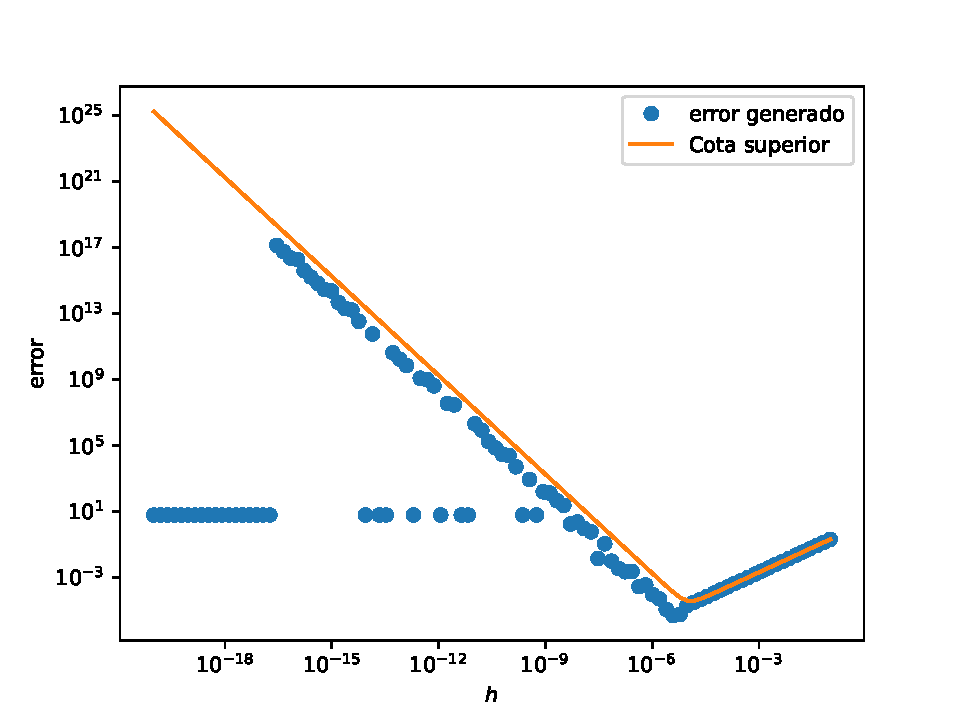
\includegraphics[width=0.5\linewidth]{contenido/img/graficodeerrorcontrol1.pdf}
    \caption{Error real y cota superior del error en la función $f(x)=x^3$}
    \label{fig:errorcontrol1}
\end{figure}
Como se aprecia en el grafico $(h,E(h))$, la cota superior del error funciona correctamente (fig \ref{fig:errorcontrol1})
